\nonstopmode
\documentclass[10pt, a4paper]{article}
%\usepackage{subfig}

\parindent=20pt
\parskip=8pt
\usepackage[width=15.5cm, left=3cm, top=2.5cm, height= 24.5cm]{geometry}
\usepackage[spanish]{babel}
\usepackage[utf8]{inputenc}
\usepackage{fancyhdr}
\usepackage{multirow}
\usepackage{rotating}
\usepackage{indentfirst}
\usepackage{latexsym}
\usepackage{caratula}
\usepackage{gnuplottex}
\usepackage{epsfig}
\usepackage{lastpage}
\usepackage{amsfonts}
\usepackage{listings}
\usepackage[export]{adjustbox}
\usepackage{pdfpages}
\lstset{language=C}
\usepackage[ruled,vlined,linesnumbered]{algorithm2e}
\usepackage{graphicx}
\usepackage{float}
\usepackage{color}

\graphicspath{{imgs/}}



% Acomodo fancyhdr.
\pagestyle{fancy}
\thispagestyle{fancy}
\addtolength{\headheight}{1pt}
\lhead{Algoritmos y Estructuras de Datos III}
\rhead{TP3}
\cfoot{\thepage /\pageref{LastPage}}
\renewcommand{\footrulewidth}{0.4pt}
\renewcommand{\thesubsubsection}{\thesubsection.\alph{subsubsection}}


\author{Algoritmos y Estructuras de Datos III, DC, UBA.}
\date{}
\title{}

\begin{document}
	
\thispagestyle{empty}
\materia{Algoritmos y Estructuras de Datos III}
\submateria{Trabajo Pr\'actico N$^{\circ}$3}
\titulo{}
\integrante{Izcovich, Sabrina}{550/11}{sizcovich@gmail.com}
\integrante{Garcia Marset, Matias}{356/11}{matiasgarciamarset@gmail.com}
\integrante{Orellana, Ignacio}{229/11}{nacho@foxdev.com.ar}
\integrante{Vita, Sebastián}{149/11}{sebastian\_vita@yahoo.com.ar}

\maketitle

\tableofcontents
\newpage

\section{Introducci\'on}
Este trabajo práctico consiste en la resolución de ciertos problemas algorítmicos que cumplen con restricciones impuestas por la cátedra, como por ejemplo el orden de complejidad máximo de los mismos, entre otras. Para justificar las implementaciones de los problemas en cuestión, fue necesaria la utilización de herramientas lógico-matemáticas que serán mencionadas a lo largo del desarrollo de cada ejercicio.\newline
Para comprobar que nuestras soluciones resolvieran correctamente los problemas propuestos, debimos dividir el análisis de los mismos en secciones a fin de estudiar minuciosamente las características de éstos. Estas secciones se dividen de la siguiente forma:

\begin{itemize}
\item \textbf{Problema a resolver:} En esta sección, nos encargamos de describir detalladamente el problema a resolver dando ejemplos del mismo y sus soluciones.
\item \textbf{Resolución coloquial:} En esta parte, nos dedicamos a explicar de forma clara, sencilla, estructurada y concisa las ideas desarrolladas para la resolución del problema en cuestión. Para ello, decidimos utilizar pseudocódigo y lenguaje coloquial combinando ambas herramientas de manera adecuada.
\item \textbf{Demostración de correctitud:} Utilizamos este apartado para justificar que el punto anterior resuelve efectivamente el problema y demostramos formalmente la correctitud del mismo.
\item \textbf{Complejidad del algoritmo:} En esta sección, nos ocupamos de deducir una cota de complejidad temporal del algoritmo propuesto en función de los parámetros considerados como correctos. Por otro lado, justificamos por qué el algoritmo desarrollado para la resolución del problema cumple con la cota dada.
\item \textbf{Instancias posibles:} Este sector presenta un conjunto de instancias que permiten verificar la correctitud del programa implementado cubriendo todos los casos posibles y justificando la elección de los mismos. Dichas instancias fueron evaluadas por el algoritmo realizado y los resultados obtenidos fueron comprobados.
\item \textbf{Experimentación:} Por último, los tests consistieron en experimentaciones computacionales utilizadas para medir la performance del programa implementado. Para ello, debimos preparar un conjunto de casos de test que permitieran observar los tiempos de ejecución en función de los parámetros de entrada que fueran relevantes. Para ello, nos encargamos de generar instancias aleatorias como también particulares. Para que los resultados fueran visibles y claros, utilizamos una comparación gráfica entre los tiempos medidos y la complejidad teórica calculada.
\item \textbf{Código fuente:} En este apéndice, presentamos las funciones relevantes del código fuente que implementa la solución propuesta. Para ello, decidimos utilizar el lenguaje \verb*#C++# dado que éste cuenta con la librería $stl$ que proporciona las estructuras necesarias para la realización de dicha tarea.
\end{itemize}
\newpage

\section{Ejercicio 1}
En este ejercicio, nos limitamos a pensar situaciones de la vida real que pudieran ser modeladas con $cliques\ de\ máxima\ frontera$.
\begin{itemize}

\item La conocida empresa internacional \textit{Chumbawamba} decide formar un equipo de trabajo para un proyecto que cambiará el mundo. Para que éste funcione sin peleas de por medio, dicho equipo debe consistir en un grupo de personas que se conozcan entre sí. Dado que la empresa desea que el proyecto sea conocido por la mayor cantidad de gente posible (siendo el boca en boca su única forma de difusión), deciden seleccionar a sus empleados de acuerdo a un conjunto que se conozca entre sí y que, también, conozca a la mayor cantidad de gente posible fuera de la empresa. Para modelar este problema, se consideran a los nodos como personas y a las aristas como la representación de un vínculo existente entre una persona y otra.

\item Un conocido golpeador desea asistir a la mejor fiesta todos los tiempos. Debido a su tardío horario de llegada al evento, éste se percata de que no puede bailar tranquilamente en el espacio reducido que encontró. Bajo un ataque de furia decide comenzar a pegarle a la gente de forma estratégica para que, al tirar a una persona, se produzca un efecto dominó y se caigan todas las que se encuentran a menos de treinta centímetros de ésta. De este modo, lograría tirar la mayor cantidad de gente al piso y disfrutar de la fiesta tranquilo. Luego, nota que le conviene comenzar a golpear a las personas que se encuentran a menos de un metro y medio de distancia entre sí y que, además, se encuentran a menos de dicha distancia con la mayor cantidad de personas para que el alcance sea mayor. Para modelar este problema, consideramos a los nodos como personas y a las arista como la representación de que la distancia entre una persona y otra es menor a un metro y medio.  

\item En un campo casi como cualquier otro, se encuentran plantas que deben ser regadas con gran potencia para no morir. Debido a que, a medida que el agua atraviesa una planta, ésta pierde potencia, el granjero \textit{Don Omar} busca que la mayor cantidad de plantas sean regadas con la mayor potencia posible. Dado que el granjero es una persona de gran capacidad pero no posee un enorme presupuesto, decide armar una estrategia de riego para sus amadas plantas teniendo que seleccionar un único circuito. Como cuenta con un único circuito de riego en el que Ésta consiste en regar alguna planta dentro de un cí de para que se muera la menor cantidad de plantas. Para modelar este problema, se consideran a los nodos como plantas y a las aristas como caminos del sistema de riego por donde puede circular el agua. %no esta terminado

\item Juanita es una apasionada de conocer calles nuevas y desea mudarse a una ciudad que le permita seguir con su pasión. Pero Juanita trabaja en el campo, o sea que fuera de cualquier ciudad, así que se le ocurre seleccionar su próxima vivienda de acuerdo a la cantidad de calles que va a poder conocer para llegar al campo. Podemos modelar el problema como los nodos representantes de las esquinas y las aristas las interconexiones entre éstas. Llamamos ciudad a todas las esquinas que se conectan todas con todas, luego, a una clique y campo a todo lo que se encuentra entre una ciudad y otra. Por lo tanto, se desea encontrar una ciudad con mayor frontera para que la cantidad de posibles calles nuevas a recorrer fuera de la ciudad sea la mayor.

\end{itemize}

\newpage

\section{Ejercicio 2}
\subsection{Explicación del algoritmo realizado}

Para resolver el problema de CMF de forma exacta, generamos un algoritmo encargado de recorrer todas las posibles cliques del grafo de entrada con la estrategia de $Backtracking$. Esto se debe a que no hallamos ninguna caracterización particular que nos permitiera reducir el espacio de búsqueda de cliques tal que el algoritmo ignorara una cantidad asintótica de ellas. Luego, nuestra implementación genera todas las soluciones posibles siguiendo un orden lexicográfico para evitar repetirlas. Por ejemplo, la clique $k_{2}$ formada por los nodos \{1,2\} es la misma que se forma al elegir los nodos \{2,1\}. Por lo tanto, al representar los nodos como números y formar cliques respetando su orden lexicográfico, nos ahorramos realizar repeticiones como la mencionada. 

De este modo, nuestro algoritmo comienza generando todas las cliques que contienen al nodo de menor valor numérico que no haya sido utilizado y, en cada paso, selecciona una serie de candidatos a ser agregados a la clique actual hasta que no quede ninguno. Una vez alcanzada dicha instancia, el algoritmo retrocede quitando el último nodo agregado a la clique e insertando al próximo candidato, si es que existe. El orden lexicográfico se respeta al momento de elegir los candidatos ya que sólo pueden ser seleccionados como tales aquellos cuyo valor representativo sea mayor al del último nodo agregado a la clique.

A continuación, se expone el pseudocódigo del algoritmo mencionado:\\

\underline{Variables globales:} \textbf{Conj(nodo)} $cliqueMaxima$, \textbf{Entero} $fronteraMaxima$.\\

\begin{algorithm}[H]
	\SetAlgoLined
	\caption{Algoritmo Exacto}
	\KwIn{\textbf{Grafo} $g$}
	\KwOut{\textbf{Conj(nodo)} $clique$}

	\For{nodo $v$ en $g$}{
		\textbf{Sort}(adyacentes($v$))
	}
	\textbf{Conj(nodo)} $clique = \emptyset$\\
	\textbf{Conj(nodo)} $candidatos = $ nodos($g$)\\

	Backtracking($clique$, $candidatos$)\\

	\textbf{devuelvo} $cliqueMaxima$\\

\end{algorithm}

\begin{algorithm}[H]
	\SetAlgoLined
	\caption{Backtracking}
	\KwIn{\textbf{Conj(nodo)} $clique$, \textbf{Conj(nodo)} $candidatos$, \textbf{Grafo} $g$} %esto hay que ponerlo bien
	\KwOut{\textbf{Conj(nodo)} $clique$}

	\For{$c \in candidatos$}{
		\If{\textbf{frontera}($ clique \cup \{c\} $) $> fronteraMaxima$ }{
			$cliqueMaxima = clique \cup \{c\} $\\
			$fronteraMaxima = $frontera($clique \cup \{c\}$)\\
		}
		\If{\textbf{frontera}($ clique \cup \{c\} $) $>$ \textbf{frontera}($clique$)}{
			Backtracking($ clique \cup \{c\} $, calcularCandidatos($ clique \cup \{c\} $), $g$, $c$)\\
		}
	}
\end{algorithm}

\begin{algorithm}[H]
	\SetAlgoLined
	\caption{frontera}
	\KwIn{\textbf{Conj(nodo)} $clique$, \textbf{Grafo} $g$} %esto hay que ponerlo bien
	\KwOut{\textbf{Entero} $res$}

	$res = 0$\\
	\For{\textbf{nodo} $v \in nodos(g)$}{
		$res = res + (\#adyacentes(v) - (\#clique - 1))$\\
	}

	\textbf{devuelvo} $res$\\

\end{algorithm}

\begin{algorithm}[H]
	\SetAlgoLined
	\caption{calcularCandidatos}
	\KwIn{\textbf{Conj(nodo)} $clique$, \textbf{Grafo} $g$, \textbf{Nodo} $ultimoNodoAgregado$} %esto hay que ponerlo bien
	\KwOut{\textbf{Conj(nodo)} $candidatos$}

	nodo $w$ = elemento de la $clique$\\

	$candidatos = adyacentes(w)$\\
	\ForAll{$v \in nodos(g)$ con $v \neq w$}{
		$candidatos$ = interseccion entre $adyacentes(v)$ y $candidatos$\\
	}

	quitar de $candidatos$ todos los nodos de valor menor a $ultimoNodoAgregado$

	\textbf{devuelvo} $candidatos$\\

\end{algorithm}

Incialmente, el algoritmo ordena las aristas en su representación interna del grafo. Esto permite hacer que ciertas operaciones tengan un costo temporal menor. Más específicamente, realizar la intersección entre los nodos adyacentes a dos nodos particulares tiene un costo lineal siempre y cuando los conjuntos se encuentren ordenados.

Nuestro programa comienza con la función $Algoritmo\ Exacto$ que se encarga de inicializar los valores con los que se llama a $Backtracking$. A su vez, esta última realiza las llamadas recursivas necesarias para ir buscando las diferentes cliques y sus candidatos, teniendo en cuenta el orden lexicográfico mencionado anteriormente. Al realizar dicho procedimiento, el algoritmo verifica en cada paso que las cliques que va considerando sean mejores que la mejor encontrada hasta el momento. Si esto no ocurre, quita el nodo en cuestión y deja de explorar cliques conteniéndolo.\\
\newline
Por otra parte, la función $calcularCandidatos$ busca aquellos nodos no contenidos en la clique en exploración pero conectados con todos los que se encuentran en ella. Dicho procedimiento se logra encontrando la intersección entre todos los nodos adyacentes a los nodos de la clique mencionada.\\
\newline
Por otro lado, la función $frontera$ devuelve la cantidad de aristas de la frontera de una clique. Para efectuar dicho cálculo, se realiza la resta de la cantidad de nodos adyacentes a cada nodo de la clique menos la cantidad de nodos de ésta menos 1, lo que sería ($\forall v \in clique$) $\#adyacentes(v)-(\#nodos(clique)-1)$. La precondición de $frontera$ consiste en que los nodos del conjunto ingresado como parámetro sean todos adyacentes entre sí.

\subsection{Complejidad Temporal}

La complejidad temporal del algoritmo exacto realizado se encuentra acotada por la complejidad de la función de $Backtracking$. Esto se debe a que para realizar el árbol de soluciones del algoritmo, se debe revisar una cantidad exponencial de opciones y dicha complejidad es mayor a la de las demás operaciones realizadas (de orden polinómico). Además, el algoritmo encuentra su solución llamando a la función $Backtracking$, lo que significa que todo lo que suceda dentro de ella se multiplica por la cantidad de llamadas a la misma. Luego, la complejidad temporal del algoritmo se puede analizar a partir del árbol de soluciones del problema en cuestión, donde cada nodo representa a una clique cuya cantidad de nodos se encuentra determinada por el nivel en el que éste se ubica. Luego, la raíz es el único caso posible de 0 nodos, el primer nivel presenta todas las posibles cliques conteniendo un único nodo y así sucesivamente con todas las posibles combinaciones. Dado que buscamos cliques compuestas por 1 a $n$ nodos, encontrar las de tamaño $k$, con $k\leq n$, tiene un costo de $\mathcal{O}({n \choose k})$ = $\mathcal{O}(\frac{n!}{(n-k)!k!})$, siendo $\frac{n!}{(n-k)!k!} \leq n^k$. Por tanto, la cantidad de pasos de dicho procedimiento resulta $\sum\limits_{i=1}^n {n \choose i} = 2^n - 1$. 

Luego, podemos determinar que la complejidad de nuestro algoritmo exacto resulta $\mathcal{O}(2^n - 1) * \ costo\ de\ realizar\ cada\ paso$.

Veamos cuál es el costo de realizar cada paso:
\begin{itemize}
\item La función $calcularFrontera$ realiza un ciclo con la cantidad de nodos, en $\mathcal{O}(n)$, que es calculada con $size() (\mathcal{O}(1))$. En dicho ciclo, se le suma a un entero ($res$) el valor de un vector ($g$) al que se accede para, luego, acceder a otro ($nodos$) y se le resta 1 a este último. Esto se realiza en $\mathcal{O}(1)*\mathcal{O}(1)$ = $\mathcal{O}(1)$. Luego, la complejidad de dicha función resulta $\mathcal{O}(n)*\mathcal{O}(1)$ = $\mathcal{O}(n)$.
\item Por otro lado, la función $interseccionNAdyacentes$ comienza creando un vector ($v\_interseccion$), cuya complejidad temporal es $\mathcal{O}(n)$\footnote{http://www.cplusplus.com/reference/vector/vector/vector/} pues consiste en un constructor por copia, y un vector $v\_tmp$ por default en $\mathcal{O}(1)$. Luego, realiza un ciclo iterando la cantidad de nodos ($indices$) recibidos por parámetro, siendo $\#indices \leq n$. En dicho ciclo, ejecuta la función $set\_intersection$ ($\mathcal{O}(2*(n+n)-1)$ este costo reequiere que los conjuntos que van a ser intersecados esten ordenados en su representación interna, esto está garantizado al principio del algoritmo ordenando los vectores que representan a los nodos adyacentes de cada nodo. \footnote{http://www.cplusplus.com/reference/algorithm/set\_intersection/?kw=set\_intersection}). Para dicha ejecución, toma el primer y último elemento de $v\_intersection$ con $begin()$ ($\mathcal{O}(1)$\footnote{http://www.cplusplus.com/reference/vector/vector/begin/}) y $end()$ ($\mathcal{O}(1)$\footnote{http://www.cplusplus.com/reference/vector/vector/end/}), como también el $back\_inserter$ de $v\_temp$ ($\mathcal{O}(n)$) y el primer y último elemento del arreglo $g$ en la posicion $indices(i)$. Dado que éstos últimos son accesos a arreglos, se realizan en $\mathcal{O}(1)$. Luego, la complejidad temporal de dicho ciclo resulta $\mathcal{O}(n)*5\mathcal{O}(1)*\mathcal{O}(n)$ = $\mathcal{O}(n^2)$.\newline
\newline
Por otro lado, se crea una cola por default en $\mathcal{O}(1)$\footnote{//www.cplusplus.com/reference/queue/queue/queue/} y, luego, se llama a un nuevo ciclo que recorre el vector $v\_intersection$ (cuyo peor caso es $\mathcal{O}(n)$). Dentro de dicho ciclo, se realiza una comparación entre un elemento de $indices$ y uno de $v\_interseccion$ ($\mathcal{O}(1)$ pues los accesos son $\mathcal{O}(1)$ cada uno y la comparación es $\mathcal{O}(1)$). Por otro lado, se realiza también un $push()$ ($\mathcal{O}(n)$\footnote{//www.cplusplus.com/reference/queue/queue/push/}). Luego, la complejidad temporal de dicho ciclo resulta $\mathcal{O}(n)*\mathcal{O}(1)*\mathcal{O}(1)$ = $\mathcal{O}(n)$.\newline
\newline
Finalmente, podemos concluir que la complejidad temporal de la función $interseccionNAdyacentes$ es $\mathcal{O}(n^2)$.
\item La función $backtracking$ comienza con la asignación a un entero de la frontera de $clique$, utilizando la función $calcularFrontera$ ($\mathcal{O}(n)$).\newline
\newline
Luego, se procede revisando si la cola $candidatos$ se encuentra vacía ($empty()$\footnote{http://www.cplusplus.com/reference/queue/queue/empty/}), en cuyo caso se le suma uno al tamaño de $clique$ ($\mathcal{O}(n)$\footnote{http://www.cplusplus.com/reference/vector/vector/resize/}).\newline
\newline
Por último, la función realiza un ciclo que itera (siempre que $candidatos$ no sea vacío) asignándole a $clique(tamaño-1)$ una referencia al siguiente elemento de candidatos con $front()$ ($\mathcal{O}(1)$\footnote{http://www.cplusplus.com/reference/queue/queue/front/}) y luego popeando $candidatos$ con $pop()$ ($\mathcal{O}(1)$\footnote{http://www.cplusplus.com/reference/queue/queue/pop/}). También, se calcula nuevamente la frontera de $clique$ y se realiza una comparación entre ésta y un entero ($\mathcal{O}(1)$) que implica una serie de asignaciones a variables enteras. Por último, se compara dicha frontera con un entero y termina por llamar recursivamente a la función $backtracking$ con $interseccionNAdyacentes$ de la nueva $clique$ formada durante la ejecución. Dichas llamadas recursivas son las que elevan la complejidad temporal del algoritmo a $\mathcal{O}(2^n - 1)$ por lo mencionado anteriormente.
\item Finalmente, la función $exacto$ crea por default un vector y una cola ($\mathcal{O}(1)$) y ejecuta un ciclo con el tamaño de $g$ (cuyo peor caso es $n$) en el que ordena ($\mathcal{O}(nlog(n))$\footnote{http://www.cplusplus.com/reference/algorithm/sort/?kw=sort})
el primer y último elemento del $i$-ésimo elemento de $g$. Luego, realiza un $push()$ de $candidatos$.\newline
\newline
Por otra parte, llama a la función $backtracking$ ($\mathcal{O}(2^n - 1)$) y, finalmente, recorre la solución obtenida para devolverla.
\end{itemize}

Finalmente, podemos afirmar que la complejidad temporal de nuestro algoritmo exacto resulta $\mathcal{O}(2^n - 1) * (\mathcal{O}(n) + \mathcal{O}(n^2))$ = $\mathcal{O}((2^n - 1) * n^{2})$ = $\mathcal{O}(n^{2}^*2^n)$.

\subsection{Experimentación}

Para las pruebas de complejidad empírica, utilizamos los tests aleatorios proporcionados por la cátedra dado que los casos del mismo son variados y no se focaliza en grafos particulares. Las mediciones de tiempo en nanosegundos se realizaron con la función $high\ resolution\ clock$\footnote{http://en.cppreference.com/w/cpp/chrono/high\_resolution\_clock} de la librería $Chrono$ de $C++$. 

Las funciones de complejidad con las que se compararon nuestros gráficos de tiempo fueron ajustadas por algoritmos matemáticos (proporcionados por \textbf{sci davis}). Dichos algoritmos se encargaron de multiplicarle y sumarle constantes a las funciones con el fin de que éstas se ajustaran a nuestros resultados sin modificar el comportamiento de las funciones utilizadas para comparar.
	
\begin{figure}[H] %[h] Aqui [b] para button [t] para top
\begin{center}
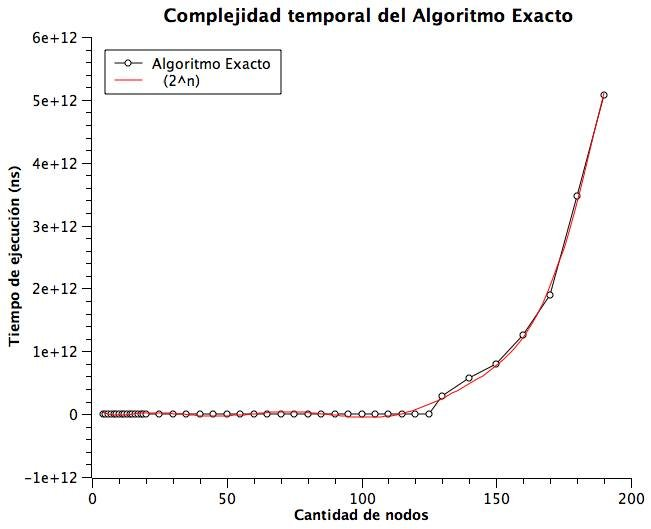
\includegraphics[width=350pt]{../imgs/exactoComplejidad.jpg}
\end{center}
\end{figure}

Como puede observarse en el gráfico anterior, la complejidad de nuestro algoritmo exacto se encuentra acotada por una función exponencial.

\newpage

\section{Ejercicio 3}
\subsection{Heurística Constructiva Golosa}
Para resolver el algoritmo presentado anteriormente con una técnica golosa, decidimos utilizar el procedimiento que se presenta a continuación:\newline
\newline
\begin{algorithm}[H]
    \SetAlgoLined
    \caption{HeurísticaGolosa}
    \KwIn{\textbf{Entero} $cantVertices$, \textbf{Entero} $cantAristas$, \textbf{Grafo} $g$} %esto hay que ponerlo bien
    \KwOut{\textbf{Conj(nodos)} $clique$}
	Entero $nodoDeMayorGrado$ = nodoDeMasGrado($g$)\\
	Grafo $cliqueHastaAhora$ = $\emptyset$\\
	agregar($v$, $cliqueHastaAhora$)\\
	\ForAll{$u \in$ adyacentes(nodoDeMayorGrado, nodos($g$))}{
		\If{forma una clique($g$, agregar($u$, $cliqueHastaAhora$)) $\land$ frontera($g$, agregar($u$, $cliqueHastaAhora$) $>$ frontera($cliqueHastaAhora$)}{
		agregar($u$, $cliqueHastaAhora$)}}
\textbf{devolver} $cliqueHastaAhora$
\end{algorithm}

donde $nodoDeMasGrado$ consiste en una función que toma el nodo del grafo cuyo grado es el mayor, $frontera$ es una función que calcula la frontera de un conjunto de nodos dentro de un grafo y $adyacentes$ consiste en una lista de nodos adyacentes a un determinado nodo.\newline


Hay que decir que es asíntico, que se rompe muy fácil, como por ejemplo cuando la clique de maxima frontera no contiene al nodo de mayor grado.

\subsection{Heurística de Búsqueda Local}

Los algoritmos de búsqueda local parten de una solución inicial $S_{0}$ y en cada paso intentan mejorarla. Para esto, se calculan todas las posibles variaciones de $S_{0}$ que forman una solución al problema. Al conjunto de todas estas se lo llama vecindad. 
Estos algoritmos se ejecutan siempre y cuando exista una solución, perteneciente a la vecindad, que sea mejor a la que ya teníamos. \newline \newline
Para nuestro ejercicio, utilizamos como $S_{0}$ al nodo 1. Dicha elección se debió a que un nodo forma una clique, con lo cual es una posible solución a nuestro problema. Además, sabemos que este existe para cualquier grafo ya que la menor cantidad de nodos que se pueden ingresar en nuestro programa es uno. 
\newline Por otro lado, decidimos separar la vecindad en 3 subconjuntos y para cada uno de estos, tomar la clique de mayor frontera. Al hacer esto, nos evitamos tener que almacenar todas las posibles cliques para posteriormente elegir la mejor. Los tres subconjuntos se formaron con las cliques que cumplen lo siguiente:
\begin{itemize}
\item \textbf{Tiene todos los nodos de $S_{0}$ salvo 1:} \newline En lugar de calcular todas las posibles cliques de este subconjunto, decidimos quedarnos únicamente con la clique que se obtiene de quitarle el nodo de menor grado a $S_{0}$. Esto se debe a que la frontera de una clique se puede calcular con la siguiente formula:\newline
Sea $S_{0}$ = ($V$,$E$) y n = $|$$V$$|$
\begin{equation}
  \delta(S_{0}) = \sum_{v \in V}^{} d(v) - n*(n-1)
\end{equation}
Ahora, si quitamos un nodo $v'$ de $S_{0}$, obtenemos lo siguiente:
\begin{equation}
  \delta(S'_{0}) = \sum_{v \in V/v'}^{} d(v) - (n-1)*(n-2)
\end{equation}
Como nosotros queremos encontrar el mayor \delta$(S'_{0})$, debemos quedarnos con el que tiene la sumatoria de mayor valor ya que (n-1)*(n-2) es igual para todas las cliques. Con lo cual, el nodo que debemos eliminar para poder maximizar la sumatoria, es el de menor grado.
\item \textbf{Tiene todos los nodos de $S_{0}$ mas uno que no pertenecía a $S_{0}$:} \newline
Para poder obtener la clique de frontera máxima de este subconjunto, buscamos todos los nodos del grafo que pueden formar una clique con $S_{0}$. Para esto, contamos cuantos nodos de la clique se conectan a cada nodo del grafo. Si un nodo es alcanzado por todos los que pertenecen a $S_{0}$, entonces ese nodo forma una clique. Una vez que tenemos a todos los posibles candidatos, calculamos la frontera de cada uno y nos quedamos con la mayor.
\item \textbf{Tiene todos los nodos de $S_{0}$ salvo 1 que se lo reemplaza por otro que no estaba en $S_{0}$:} \newline
\end{itemize}
Una vez que generamos la vecindad, tomamos la clique de mayor frontera, $S_{maxima}$ y la comparamos con $S_{0}$. Si la frontera de $S_{0}$ es menor, $S_{maxima}$ es nuestra nueva solución inicial. Caso contrario, el programa finaliza ya que ningún elemento de la vecindad puede mejorarla.



%no entendi esto! 
%Hay que ver cuánto dura cada vértice en cantidad de ejecuciones.


\subsection{Heurística de Búsqueda Tabú}

\begin{algorithm}[H]
    \SetAlgoLined
    \caption{TabuSearch}
    \KwIn{\textbf{Conj(nodos)} $solución\_inicial$, \textbf{Grafo} $g$, \textbf{Entero} $cantidad\_pasos$, \textbf{Entero} $desviacion\_permitida$}
    \KwOut{\textbf{Conj(nodos)} $solución\_final$}
		
	\textbf{Entero} $desviacion\_permitida\_aux$ = 0 \\
	\textbf{Conj(nodos)} $solución\_final$ = $solución\_inicial$ \\
		
	\While{$cantidad\_pasos >$ 0}{
		\textbf{Entero} $frontera\_ini$ = frontera($solución\_inicial$) \\
	 	\For{$u \in Candidatos\_clique(g,u)$}{
	 		\If{$\neg$ es tabu($u$) $\land \neg$ esta agregado $u$ en $solución\_inicial$}{
	 			\eIf{frontera($solución\_final$) $<$ Frontera con $u$ en $solución\_inicial$}{
					$solución\_final$ = $solución\_inicial$ con $u$}{
	  				\If{$desviacion\_permitida\_aux >$ 0}{
	 				$solución\_inicial$ = $solución\_inicial$ con $u$ \\
	 				Poner en lista Tabu a $u$ \\
	 				$desviacion\_permitida\_aux$ - 1}}}}}
	
	\ForAll{$u \in$ Nodos($solución$\_$inicial$)}{
		\If{$\neg$ es tabu($u$)}{
	 		\eIf{frontera($solución\_final$) $<$ Frontera sin $u$ en $solución\_inicial$}{
	 			$solución\_final$ = $solución\_inicial$ sin $u$}{
				\If{$desviacion\_permitida\_aux >$ 0}{
					$solución\_inicial$ = $solución\_inicial$ sin $u$ \\
					Poner en lista Tabu a $u$ \\
					$desviacion\_permitida\_aux$ - 1}}}}
							
	\If{$desviacion\_permitida\_aux \leq$ 0}{
		$solución\_inicial$ = $solución\_final$}
	\While{$frontera\_ini <$ frontera($solución\_final$) $\vee \ desviacion\_permitida\_aux >$ 0}{
		$desviacion\_permitida\_aux$ = $desviacion\_permitida$ \\
		Vaciar la lista Tabu \\
		Agregar los ultimos dos nodos de $solución\_final$ a la lista Tabu \\
		$cantidad\_pasos$ - 1}
    	\textbf{devolver} $solución\_final$ \\

\end{algorithm}

Donde:
\begin{itemize}
 \item $desviacion$\_$permitida$ dice la cantidad de veces que se agrega o quita un nodo por iteracion (empeorando la solución parcial).
 \item $cantidad$\_$pasos$ son la cantidad de veces que se aplica el algoritmo. Tener en cuenta que la primera iteracion $desviacion$\_$permitida$ es 0, por lo que se toma el maximo local.
 \item frontera : Dice, dada una solución como parametro, el numero de nodos adyacentes a la frontera (es lo que pide maximizar el enunciado).
 \item Candidatos$\_$clique : Dice los nodos que pertenecen a la clique del nodo pasado como parametro.
 \item Nodos : da los nodos pertenecientes a la solución pasada como parametro.
\end{itemize}

\newpage

\section{Ejercicio 4}
%En el grafico se puede observar como el crecimiento de todos las heuristicas es polinomial a menida que el grafo aumenta su densidad en aristas. A su vez el algoritmo $Tabu$ $Search$ presenta una mayor diferencia en cuanto a tiempo, esto es razonable porque puede empeorar parcialmente la solucion dependiendo la cantidad de nodos, entonces esa diferencia (constante) lo que hace es "subirme" la funcion la cantidad observada. 

Para realizar la experimentación respecto a la calidad de las heurísticas presentadas, utilizamos un generador de las siguientes familias de grafos:
\begin{itemize}
\item Estrella + CMF
 \begin{figure}[H] %[h] Aqui [b] para button [t] para top
\begin{center}
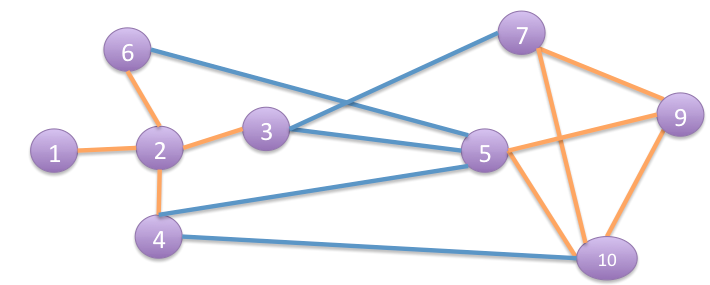
\includegraphics[width=200pt]{../imgs/Estrella+CMF.jpg}
\caption{Grafo de ejemplo de tipo Estrella con una CMF que no esta en la estrella.}
\end{center}
\end{figure}
\item Estrella+Puente+CMF
 \begin{figure}[H] %[h] Aqui [b] para button [t] para top
\begin{center}
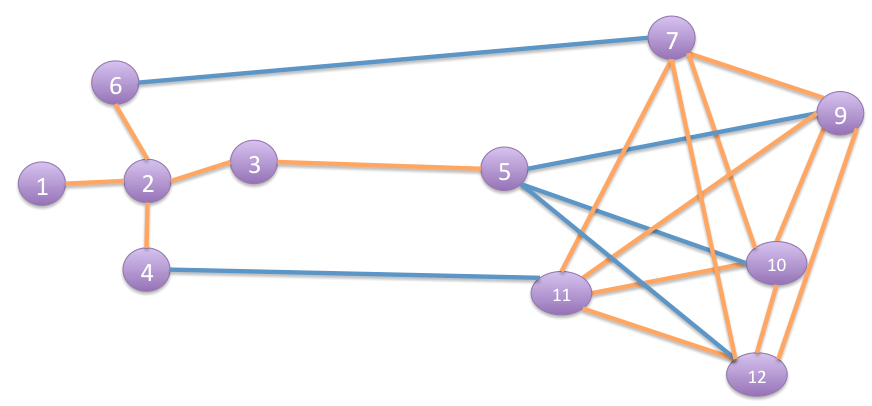
\includegraphics[width=200pt]{../imgs/Estrella+Puente+CMF.jpg}
\caption{Grafo de ejemplo de tipo Estrella con un puente a otra parte del grafo que tiene la CMF}
\end{center}
\end{figure}
\item Estrella+Puente+Doble Estrella
 \begin{figure}[H] %[h] Aqui [b] para button [t] para top
\begin{center}
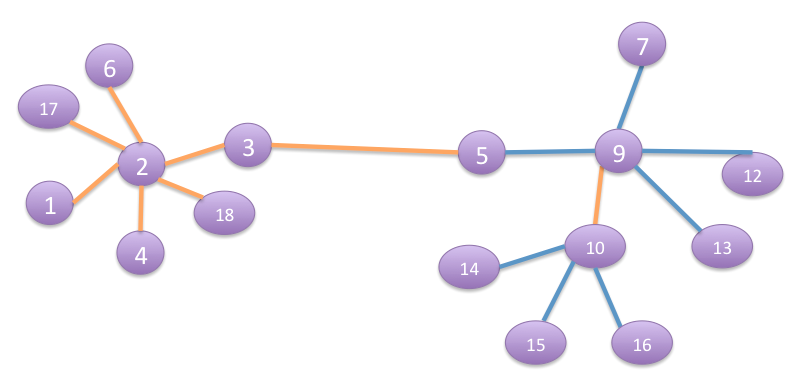
\includegraphics[width=200pt]{../imgs/Estrella+puente+dobleEstrella.jpg}
\caption{Grafo de ejemplo de tipo Estrella con un puente a una estrella doble.}
\end{center}
\end{figure}

\item Banana Tree (Palmera)
 \begin{figure}[H] %[h] Aqui [b] para button [t] para top
\begin{center}
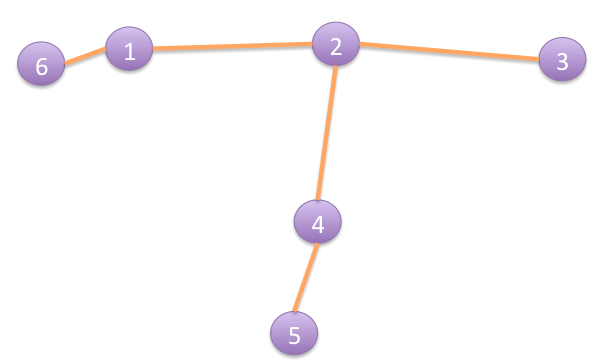
\includegraphics[width=200pt]{../imgs/banana.jpg}
\caption{Grafo de ejemplo de tipo Estrella con un puente a una estrella doble.}
\end{center}
\end{figure}
\item Rueda
 \begin{figure}[H] %[h] Aqui [b] para button [t] para top
\begin{center}
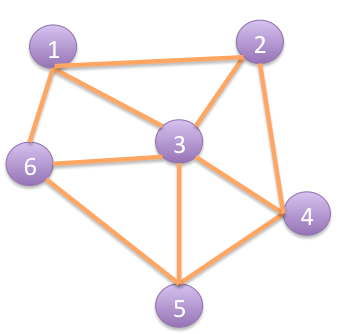
\includegraphics[width=150pt]{../imgs/rueda.jpg}
\caption{Grafo de ejemplo de tipo Estrella con un puente a una estrella doble.}
\end{center}
\end{figure}
\end{itemize}
Luego, procedimos aumentando la cantidad de nodos de los grafos, que a su vez aumenta la cantidad de aristas de éstos dado que los grafos en cuestión se caracterizan por un porcentaje determinado de aristas con respecto a sus nodos. De este modo, realizamos pruebas para cada heurística sobre cada familia de grafos.

Por otro lado, separamos las pruebas de calidad de soluciones en chicas y grandes, esto lo hicimos ya que nos interesa ver la solucion obtenida por el algoritmo exacto para poder compararlo con las heurísticas, y en otro contexto tambien comparar la calidad de las soluciones de las heurísticas para grafos donde el algoritmo exacto no puede resolver a tiempo. 

Las pruebas chicas consisten en grafos de entre 10 y 150 nodos con una densidad de aristas del 50\%. De esta forma, el algoritmo exacto puede encontrar soluciones en un tiempo relativamente rápido y nos permite compararlo con las heurísticas. En el caso de las pruebas grandes, tomamos grafos de entre 200 y 2000 nodos con una densidad de aristas del 50\%. La decisión acerca de la cantidad de aristas se realizó de forma tal a encontrar un balance entre grafos con pocas y muchas aristas, sin afectar demasiado el tiempo de ejecución del algoritmo exacto y de las heurísticas. 


 \begin{figure}[H] %[h] Aqui [b] para button [t] para top
\begin{center}
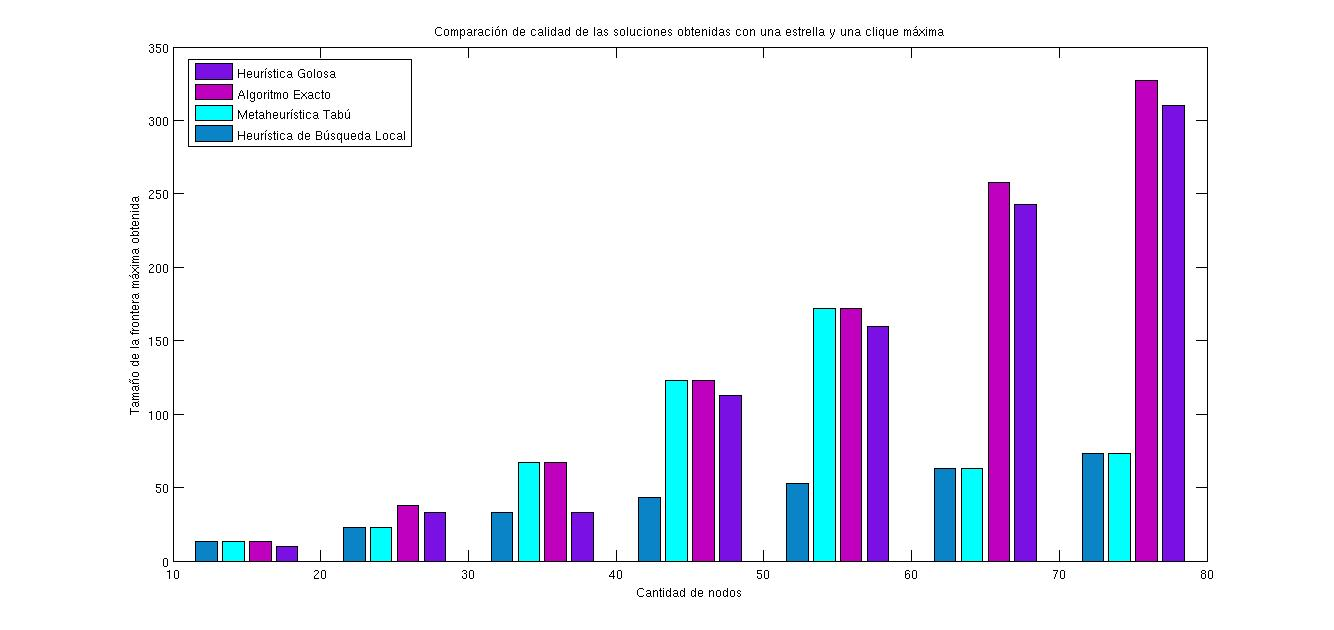
\includegraphics[width=400pt]{../imgs/calidadSolucionesChicas15.jpg}
\caption{Comparación realizada con soluciones chicas con un grafo de tipo Estrella+CMF.}
\end{center}
\end{figure}

En este caso, tenemos una estrella cuyo nodo central no forma parte de la clique de frontera máxima, con lo cual aquellos algoritmos que consideren a los nodos de mayor grado para empezar su ejecución y llegar a un resultado se verán perjudicados por esta familia. Tanto la heurística de búsqueda local como la metaheurística Tabú se ven perjudicadas por la caracterización del grafo, esto se debe a que la heurística parte del nodo de mayor grado y se mueve por una vecindad pequeña y nunca llega a encontrar la CMF que se encuentra a una distancia considerable de la estrella que forma el nodo. En el caso de la metaheurística, lo que sucede es que parte de una solución incial dada por la búsqueda local, con lo cual tiene un punto de partida poco ventajoso que termina provocando que genere un mal resultado. En el caso de la búsqueda golosa, esta se ve beneficiada ya que si bien empieza con el nodo de mayor grado, eventualmente prueba con otros nodos teniendo asá mayor probabilidad de encontrar la clique de frontera máxima. 

 \begin{figure}[H] %[h] Aqui [b] para button [t] para top
\begin{center}
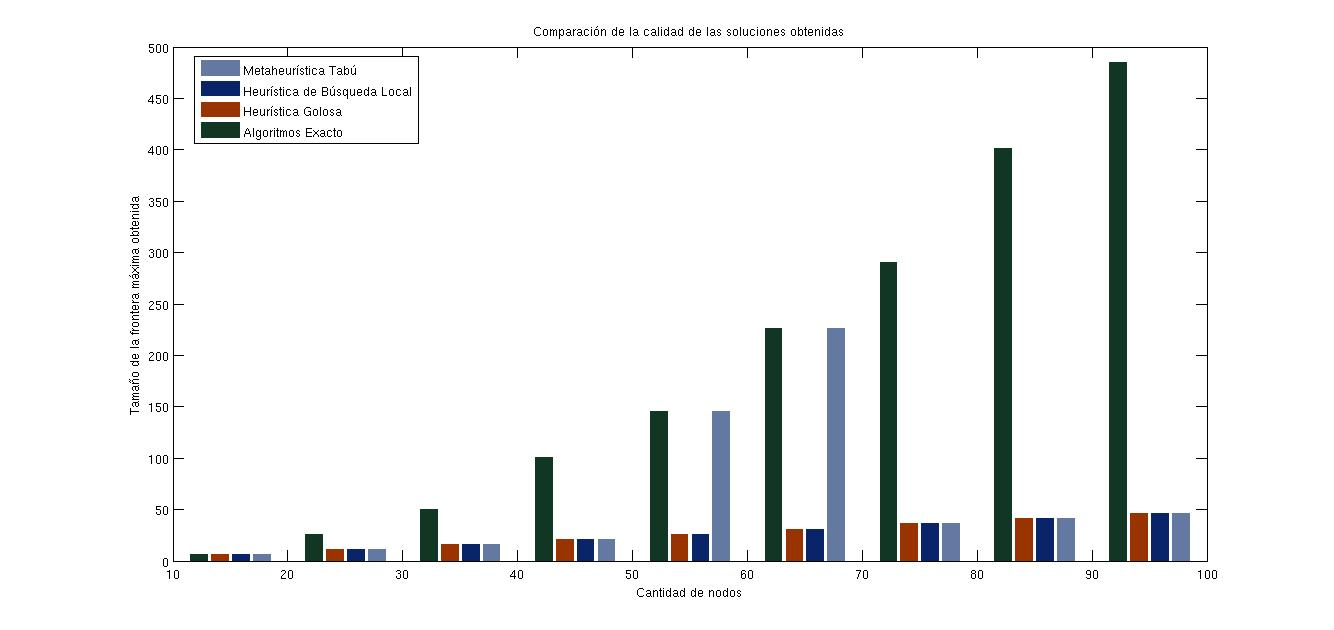
\includegraphics[width=400pt]{../imgs/calidadSolucionesChica14.jpg}
\caption{Comparación realizada con soluciones chicas con un grafo de tipo Estrella+Puente+CMF.}
\end{center}
\end{figure}



En este caso sucede lo mismo que en el anterior, los algoritmos inician en la estrella ya que ésta tiene mayor grado y provoca que nunca se logren mover hasta las soluciones que se encuentran del otro lado del puente que se forma entre la estrella y la estructura que contiene una clique de frontera máxima del otro lado.

 \begin{figure}[H] %[h] Aqui [b] para button [t] para top
\begin{center}
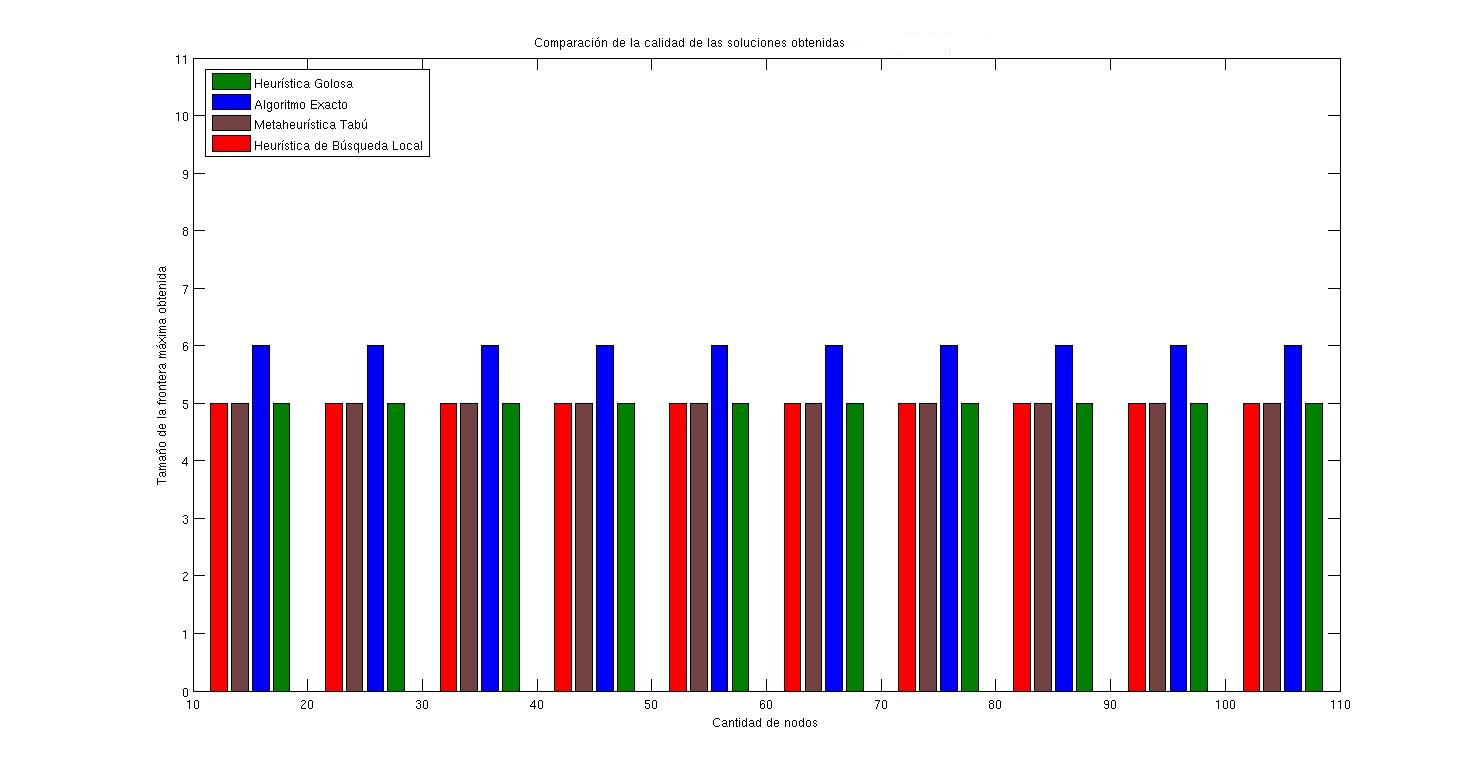
\includegraphics[width=400pt]{../imgs/calidadSolucionesChicas17.jpg}
\caption{Comparación realizada con soluciones chicas con un grafo de tipo Estrella+Puente+Doble Estrella.}
\end{center}
\end{figure}


En este caso, el grafo se caracteriza por contener una estrella que está conectada con dos estrellas. Estas dos estrellas forman una clique de frontera maxima que no contiene al nodo de la primera estrella. Lo que sucede es que la solución de la estrella es parecida a la solucion correcta del problema, pero esta no es la mejor que encuentra el exacto, por eso las heurísticas se quedan con ella mientras que el exacto encuentra la mejor solución entre las estrellas que estan unidas.


 \begin{figure}[H] %[h] Aqui [b] para button [t] para top
\begin{center}
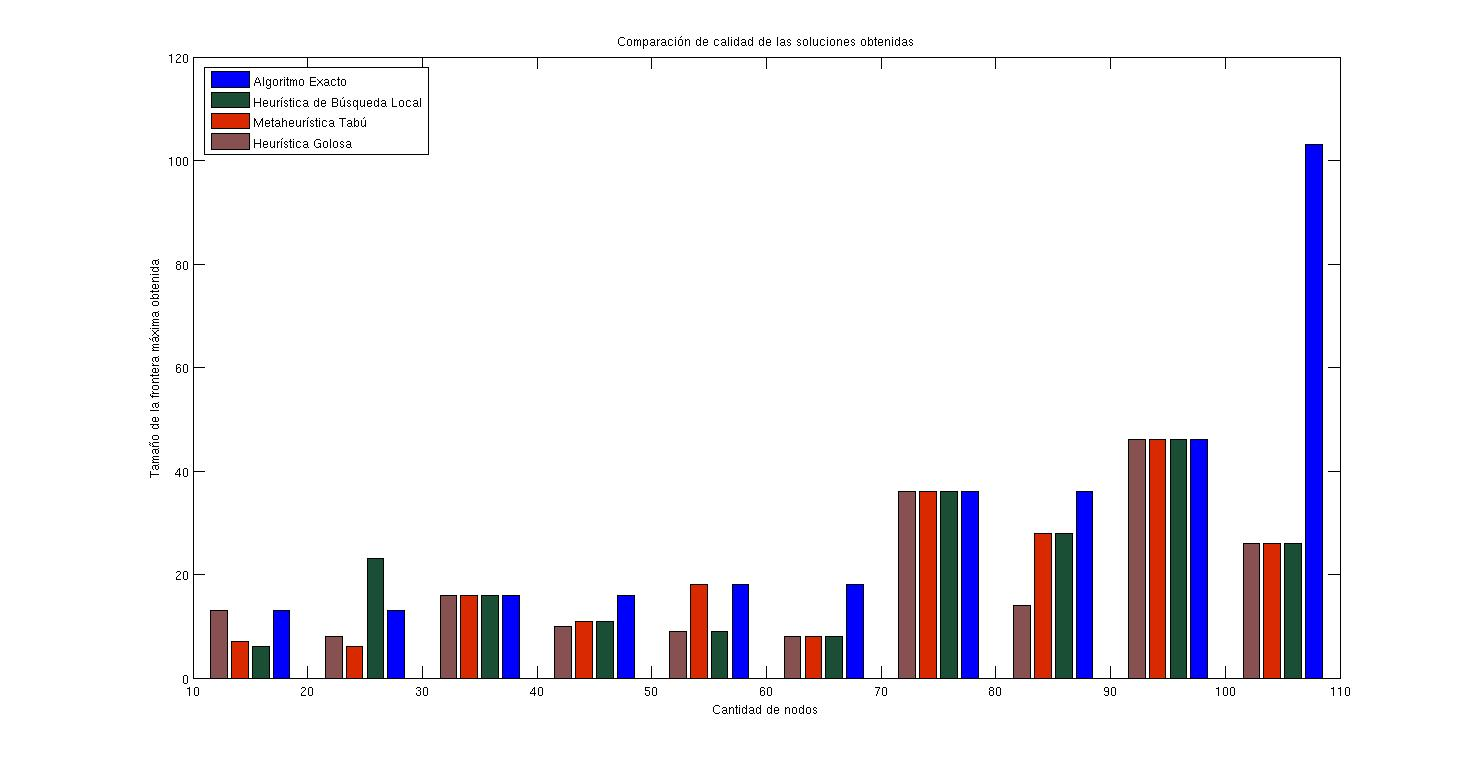
\includegraphics[width=400pt]{../imgs/calidadSolucionesChicas3.jpg}
\caption{Comparación realizada con soluciones chicas con un grafo de tipo Banana Tree.}
\end{center}
\end{figure}

En este caso, tenemos un grafo de tipo banana tree, las heurísticas en la mayoría de los casos obtuvieron soluciones correctas.

 \begin{figure}[H] %[h] Aqui [b] para button [t] para top
\begin{center}
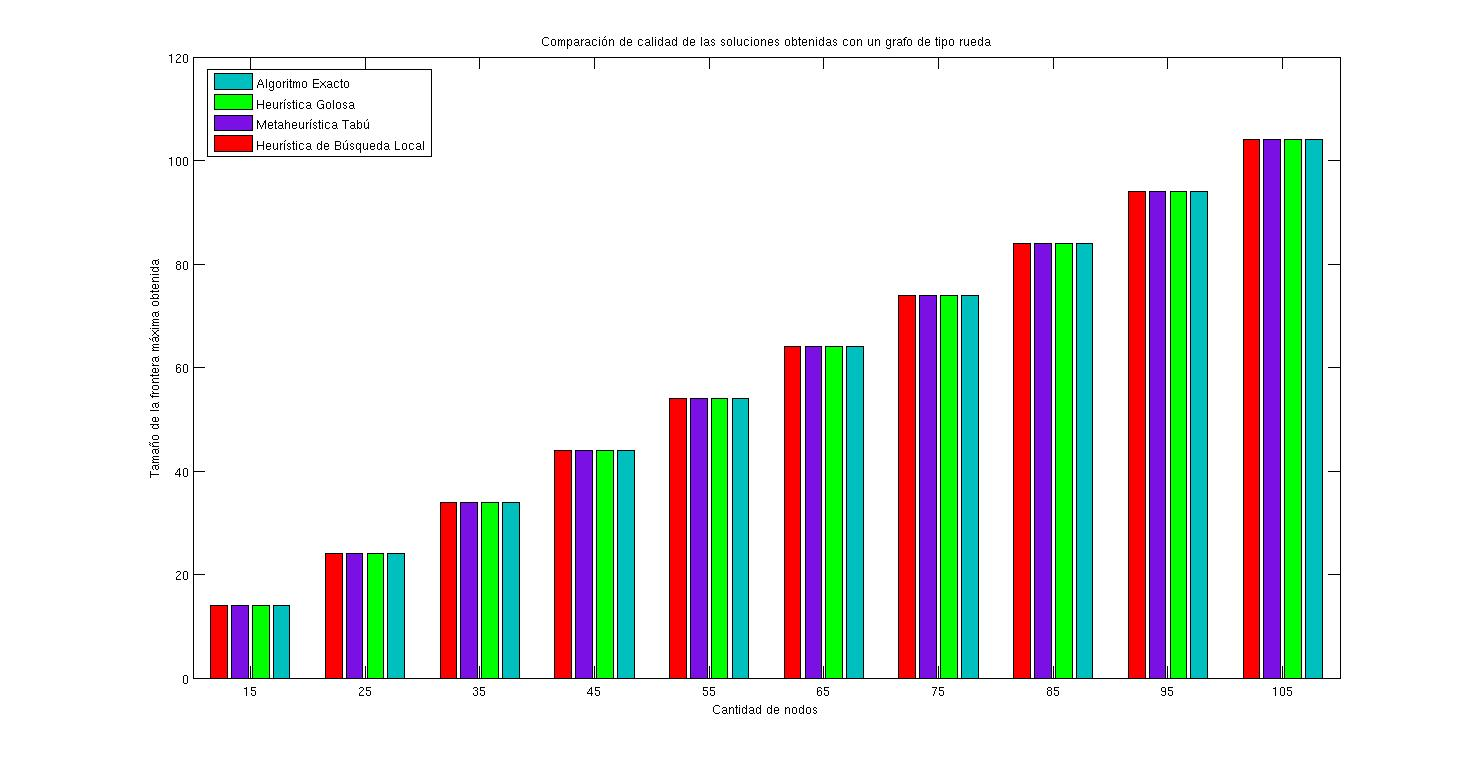
\includegraphics[width=400pt]{../imgs/calidadSolucionesChicas2.jpg}
\caption{Comparación realizada con soluciones chicas con un grafo de tipo rueda.}
\end{center}
\end{figure}

 \begin{figure}[H] %[h] Aqui [b] para button [t] para top
\begin{center}
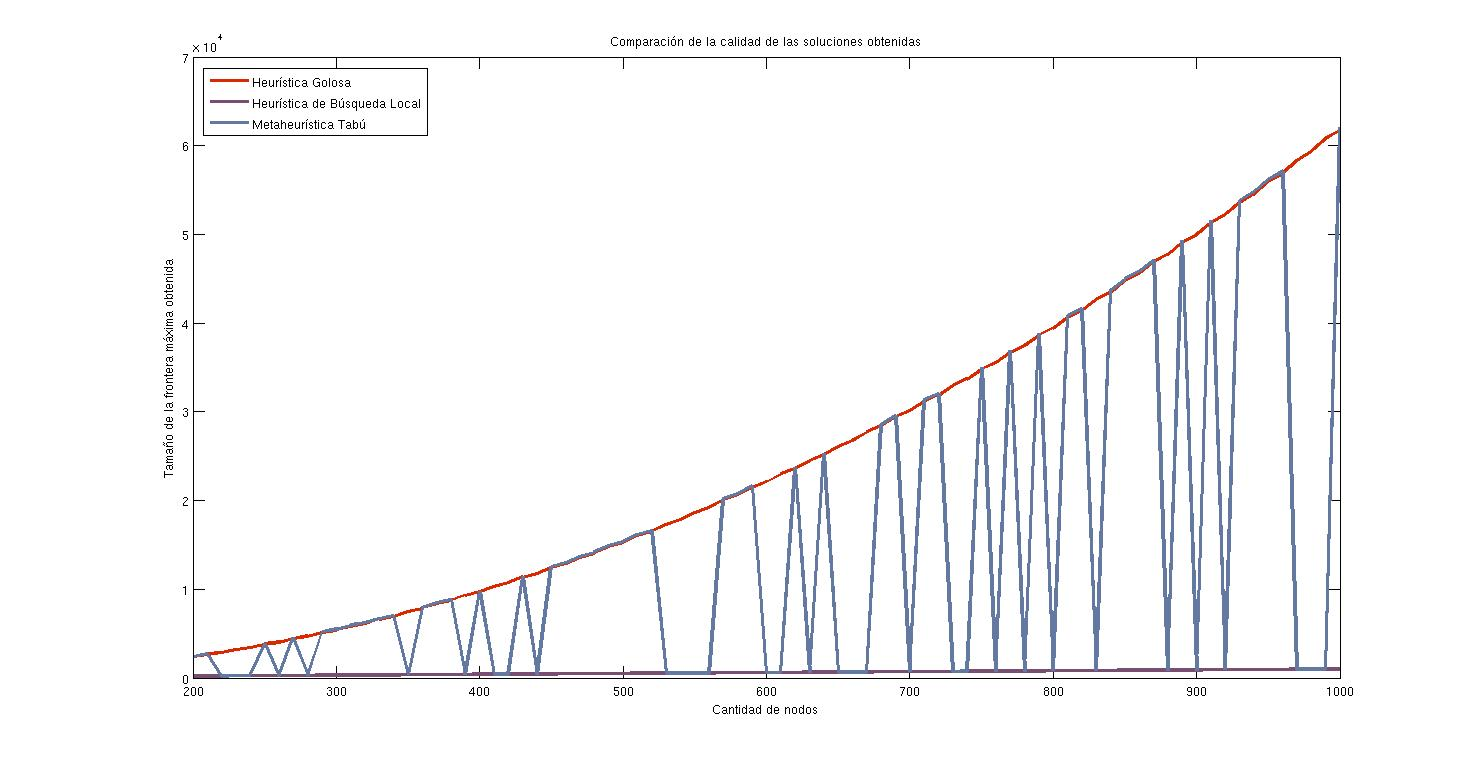
\includegraphics[width=400pt]{../imgs/calidadSolucionesGrandes15.jpg}
\caption{Comparación realizada con soluciones grandes con un grafo de tipo Estrella+CMF.}
\end{center}
\end{figure}

 \begin{figure}[H] %[h] Aqui [b] para button [t] para top
\begin{center}
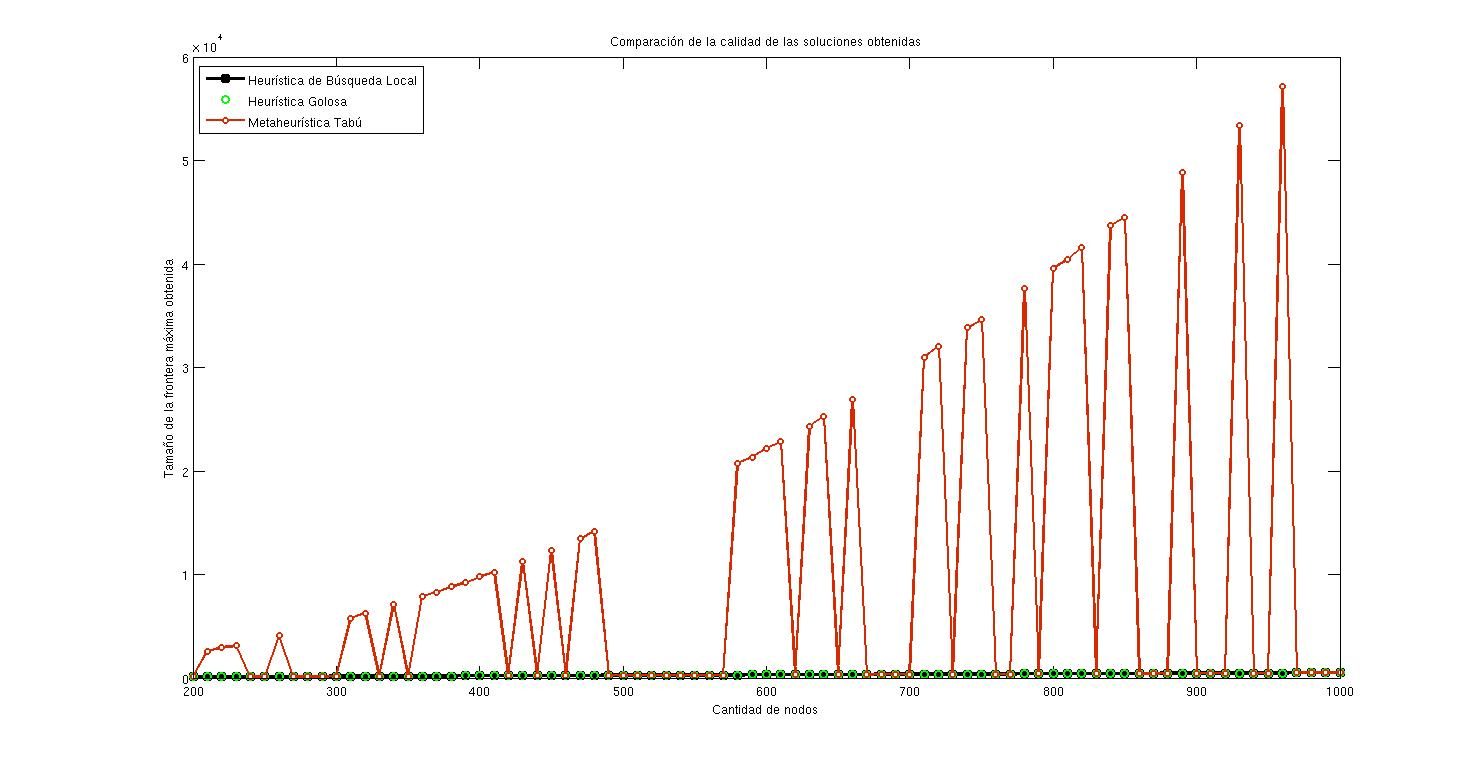
\includegraphics[width=400pt]{../imgs/calidadSolucionesGrandes14.jpg}
\caption{Comparación realizada con soluciones grandes con un grafo de tipo Estrella+Puente+CMF.}
\end{center}
\end{figure}

 \begin{figure}[H] %[h] Aqui [b] para button [t] para top
\begin{center}
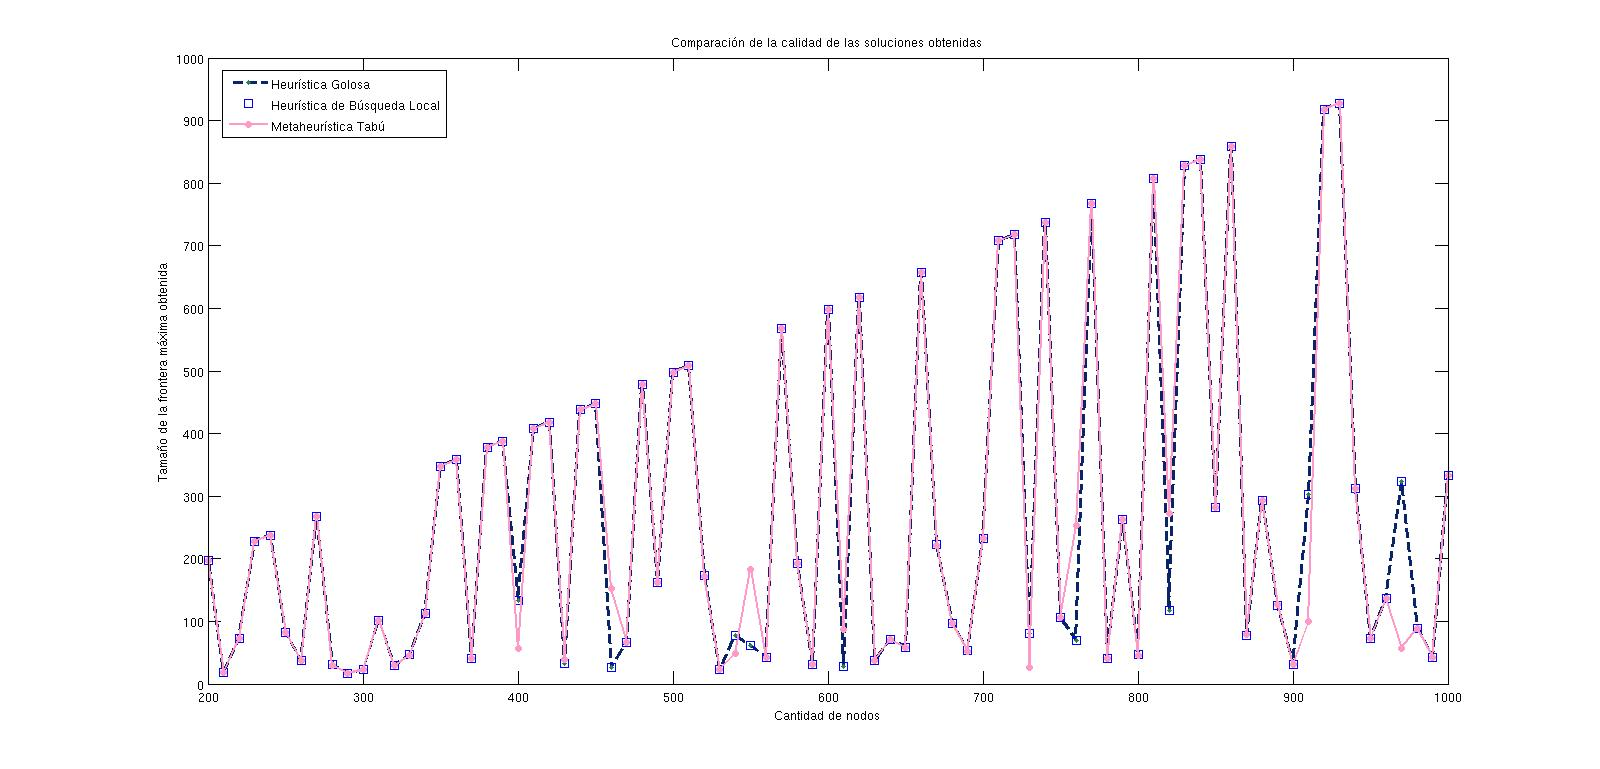
\includegraphics[width=400pt]{../imgs/calidadSolucionesGrandes3.jpg}
\caption{Comparación realizada con soluciones grandes con un grafo de tipo Banana Tree.}
\end{center}
\end{figure}







\newpage

\section{Referencias}
\begin{itemize}
\item CORMEN, THOMAS H. ; Introduction to Algorithms, Third ed. 2009. The MIT Press.
\end{itemize}


\section{Código fuente}


\end{document}
